\chapter{Discussion}
\label{chap:discussion}
\section{Wiki-Based}
The wiki-based part of the experiment has shown none relevant or significant results. However, 
this points that for the hypothesis stated before, the reading of texts may be equally treated 
in both polarities in a wiki-based webpage. These results can lead to theories, either
the reading task was not long enough to induce difficulties or daily users are highly adapted to
both polarities due to the wide use of the internet. 


\begin{figure}[H]
    \centering
    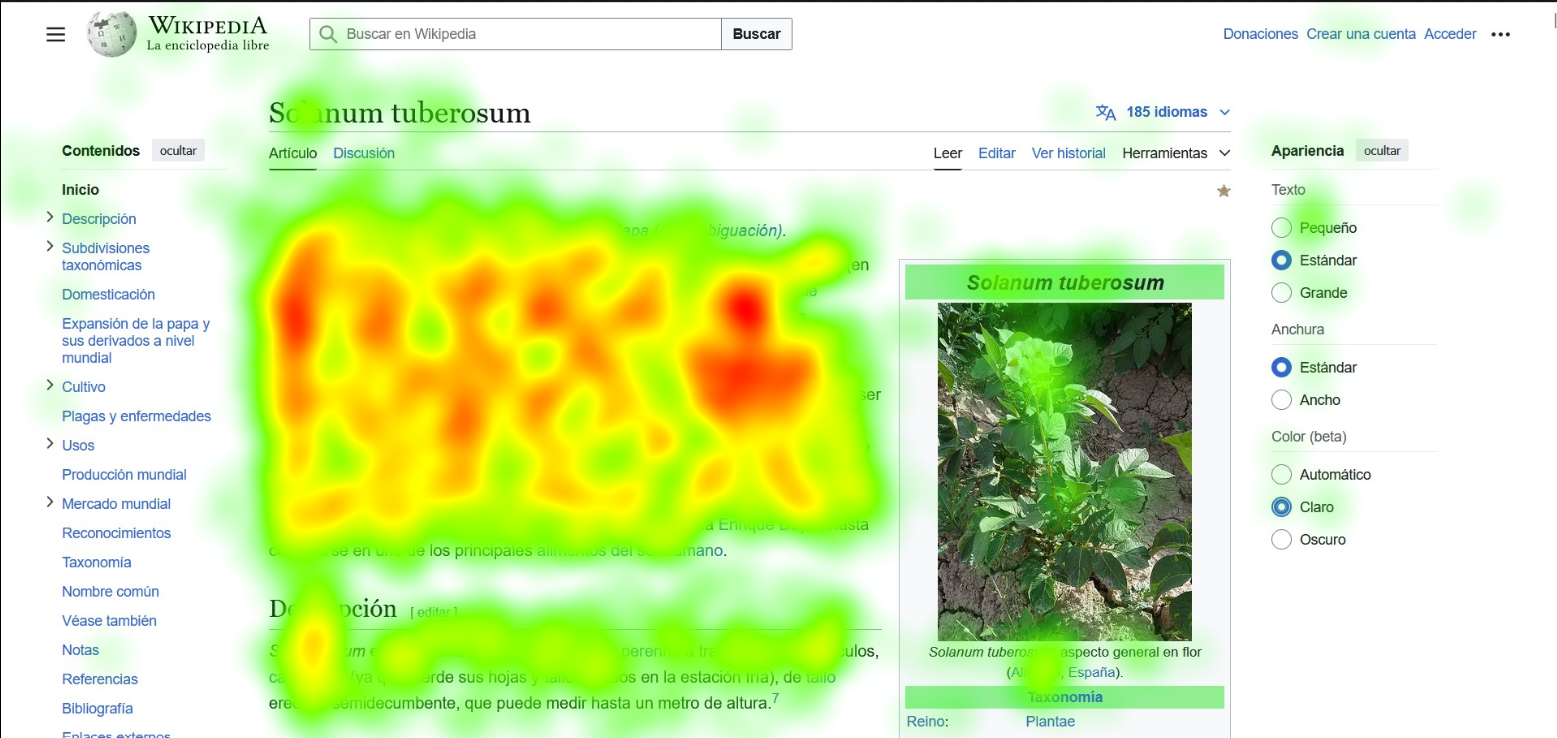
\includegraphics[width=0.85\textwidth]{figures/PaataFix.png}
    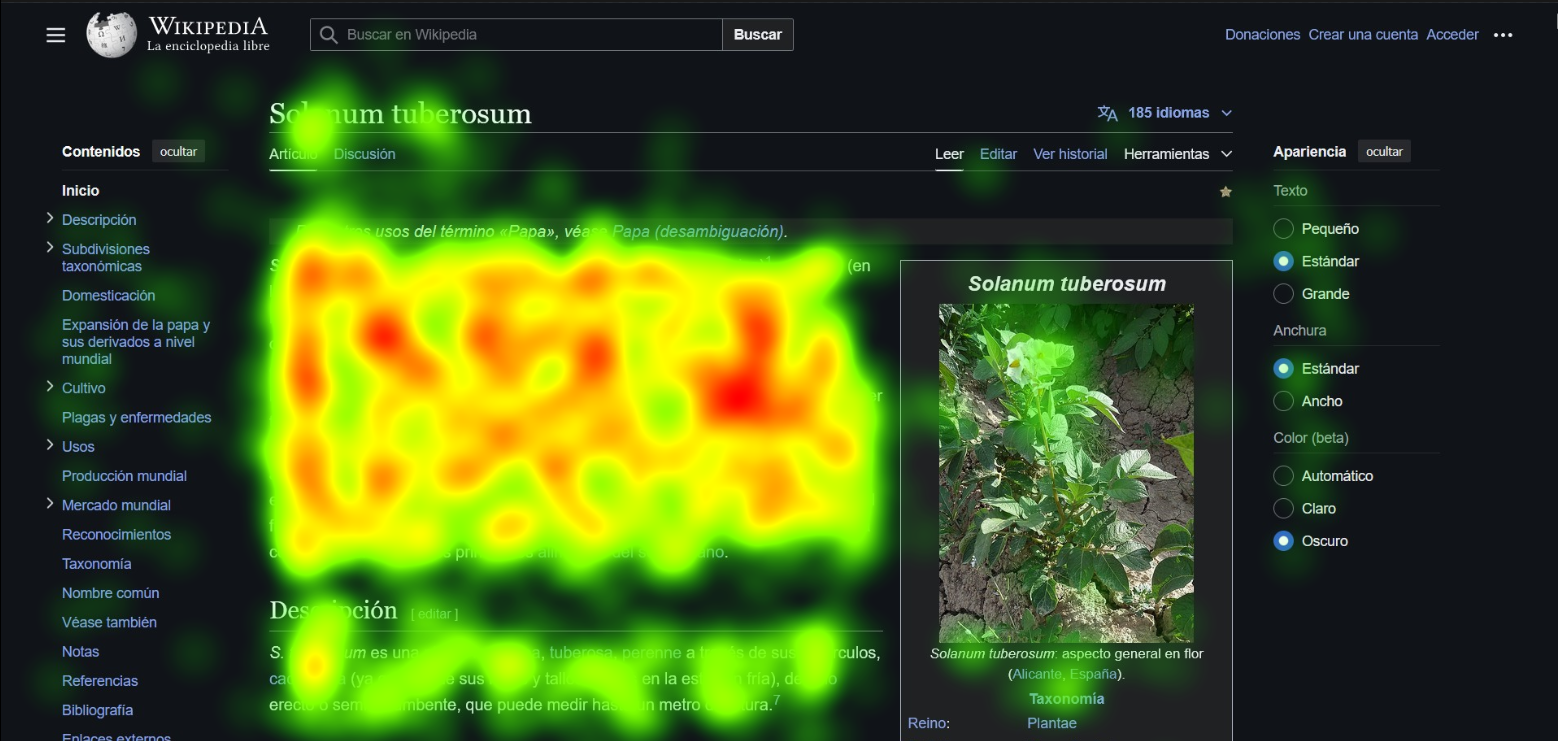
\includegraphics[width=0.85\textwidth]{figures/PatataOscFix.png}
    \caption{Fixations heatmap of wiki-based experiment. First image 
    positive polarity, second image negative polarity.}
    \label{fig:wiki-results}
\end{figure}

Regarding the preference of users in this scenario, overall users prefer positive polarity over negative polarity 
supporting the hypothesis H3.
However, when the users of negative polarity were asked the preference, the results were evenly distributed 
between both polarities and the comprehension questions had an even distribution of correct percentages.
\section{E-Commerce}
The e-commerce part has no significant results either, however there is a variable that was 
relevant and almost significant, the average duration of fixations. As expressed in the chapter \ref{chap:data_analysis}
this variable is related to the difficulty of reading this can be an indicator for the hypothesiis H1 analyzing the result
of this variable. There's proof that users may have less difficulty reading in the negative polarity
than in the positive polarity. Although as the result is not significant but relevant, more research is needed 
to confirm this hypothesis.
\begin{figure}[H]
    \centering
    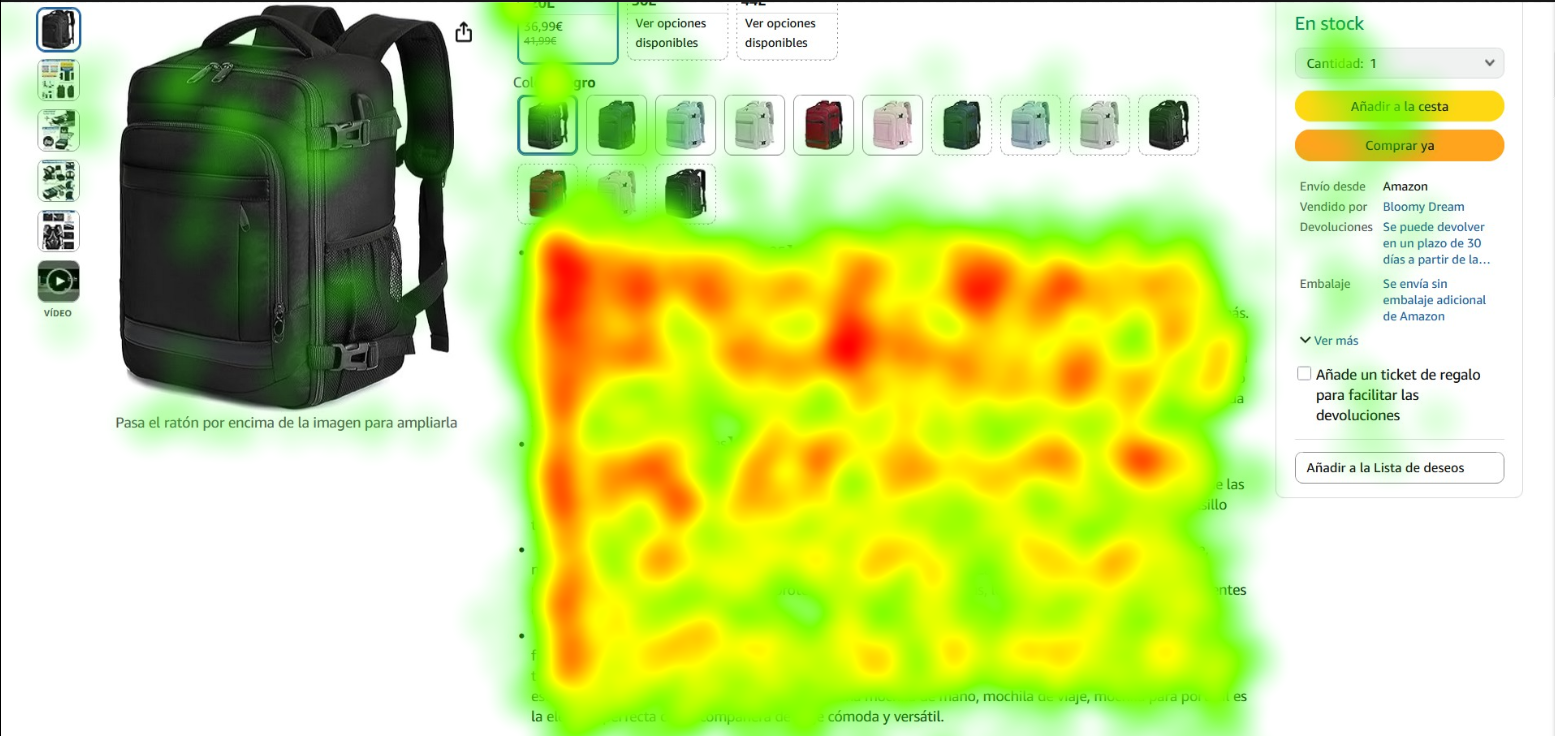
\includegraphics[width=0.8\textwidth]{figures/MochilaClarFix.png}
    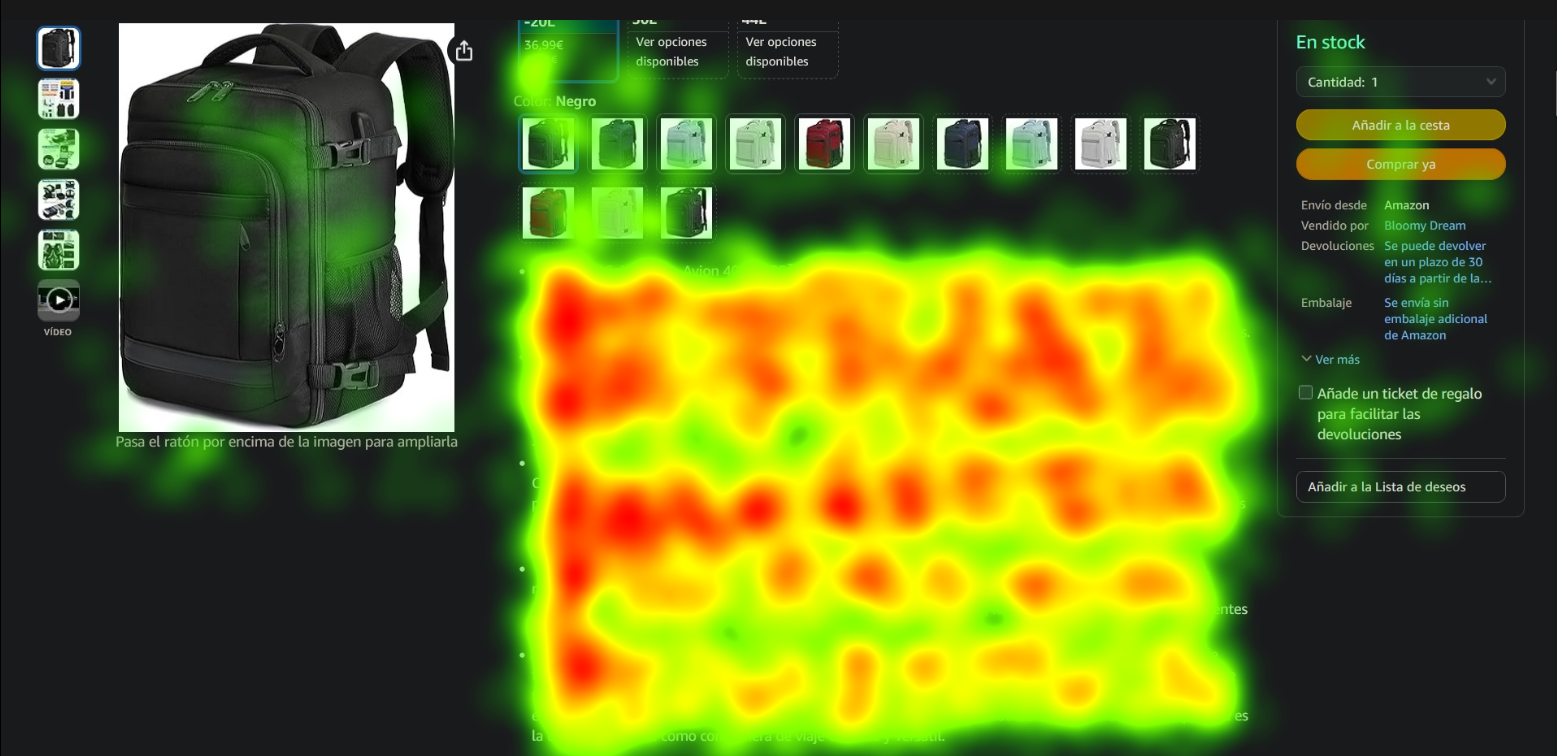
\includegraphics[width=0.8\textwidth]{figures/MochilaOscFix.png}
    \caption{Fixations heatmap of e-commerce experiment. First image 
    positive polarity, second image negative polarity.}
    \label{fig:moch-results}
\end{figure}

The reading questions had a high pecentage of correct answers in both polarities, in addition, the
preference of users was higher overall for the positive polarity with a higher difference than the wiki-based scenario.
Supporting the hypothesis H3 of users prefering positive polarity over negative polarity.
\section{Preference Questionnaires}
None of the questions regarding preference had significant results. However, the results
indicate that users used more the positive polarity daily than the negative polarity. 
Both of them shared the same percentage of users finding the webpages professional and 
appealing. Both groups agreed that the colors used in their experiment made the text
easier to read. 


